\documentclass[11pt]{elegantbook}

\title{Theoretical Problems}
\subtitle{Numerical analysis 2022}

\author{Wenchong Huang (EbolaEmperor)}
\institute{School of Mathematical Science, Zhejiang University}
\date{September 20th, 2022}

\extrainfo{ Elegantly learning. }

\logo{logo-blue.png}
\cover{cover.jpg}

% modify the color in the middle of titlepage
\definecolor{customcolor}{RGB}{32,178,170}
\colorlet{coverlinecolor}{customcolor}

\tikzset{elegant/.style={smooth,thick,samples=50,cyan}}
\tikzset{eaxis/.style={->,>=stealth}}

\usepackage{float}
\usepackage{pgfplots}
\usepackage{tikz}

\begin{document}

\maketitle

\frontmatter
% \tableofcontents

\mainmatter

\chapter{Solving Nonlinear Equations}

\begin{problem}
  Consider the bisection method starting with the initial interval $[1.5,3.5]$. In the following questions "the interval" refers to the bisection interval whose width changes across different loops.
  \begin{itemize}
    \item What is the width of the interval at the $n$th step?
    \item What is the maximum possible distance between the root $r$ and the midpoint of the interval?
  \end{itemize}
\end{problem}

\begin{solution}
  Note that the interval's width is multipled by $\frac{1}{2}$ at each step, and the initial width is $2$, hence the width \textbf{after} the $n$th step is $\frac{1}{2^{n-1}}$.
  
  The maximum distance is not grater than $1$ obviously.

  Since the loop terminated when $|f(c)|<\varepsilon$, we could construct an increasing function $f$ whose root is $1.5+\delta$, and $|f(x)|<\varepsilon$ everywhere, hence the bisection loop will terminate at first step, the distance between midpoint and root is $1-\delta$. Let $\delta\to 0^+$, we know the distance could be infynitely close to $1$.
\end{solution}

\vspace{1.5em}

\begin{problem}
  In using the bisection algorithm with its initial interval as $[a_0,b_0]$ with $a_0>0$, we want to determine the root with its relative error no grater than $\varepsilon$. Prove that this goal of accuracy is guaranteed by the following choice of the number of steps,
  \begin{equation*}
    n\geq\frac{\log(b_0-a_0)-\log\varepsilon-\log a_0}{\log 2}-1
  \end{equation*}
\end{problem}

\begin{solution}
  Suppose the root is $r\geq a_0$. The relative error \textbf{after} the $n$th step is
  \begin{equation}
    \frac{|r-c_n|}{|r|}
  \end{equation}
  
  The following inequations hold
  \begin{equation}
    \frac{|r-c_n|}{|r|} \leq \frac{\frac{1}{2}(b_n-a_n)}{r} \leq \frac{\frac{1}{2}(b_n-a_n)}{a_0} = \frac{b_0-a_0}{a_0 2^{n+1}}
  \end{equation}

  Hence when (1.1) holds, we have
  \begin{align*}
   & (n+1)\log 2 \geq \log(b_0-a_0) -\log\varepsilon -\log a_0\\
  \implies & \log 2^{n+1} \geq \log \left(\frac{b_0-a_0}{\varepsilon a_0}\right)\\
  \implies & 2^{n+1} \geq \frac{b_0-a_0}{\varepsilon a_0} \implies \frac{b_0-a_0}{a_0 2^{n+1}} \leq \varepsilon
  \end{align*}

  Hence the conclution is proved by (1.2).
\end{solution}

\vspace{1.5em}

\begin{problem}
  Perform four iterations of Newton's method for the polynomial equation $p(x)=4x^3-2x^2+3=0$ with the starting point $x_0=-1$. Use a hand calculator and organize results of the iterations in a table.
\end{problem}

\begin{solution}
Firstly we derivate $p(x)$
\begin{equation*}
  p'(x)=12x^2-4x
\end{equation*}

The results are shown as the following table.
  \begin{table}[htbp]
    \centering
    \small
    \begin{tabular}{|c|c|c|c|c|}
    \hline
    \textbf{$n$} & \textbf{$x_n$} & \textbf{$p(x_n)$} & \textbf{$p'(x_n)$} & \textbf{$x_n-\frac{f(x_n)}{f'(x_n)}$} \\ \hline
    \textbf{0}   & -1             & -3                & 16                 & -0.8125                               \\ \hline
    \textbf{1}   & -0.8125        & -0.46582          & 11.1719            & -0.770804                             \\ \hline
    \textbf{2}   & -0.770804      & -0.0201359        & 10.2129            & -0.768832                             \\ \hline
    \textbf{3}   & -0.768832      & -3.98011e-05      & 10.1686            & -0.768828                             \\ \hline
    \textbf{4}   & -0.768828      &                   &                    &                                       \\ \hline
    \end{tabular}
  \end{table}
\end{solution}

\begin{problem}
  Consider a variation of Newton's method in which only the derivative at $x_0$ is used,
  \begin{equation}
    x_{n+1}=x_n-\frac{f(x_n)}{f'(x_0)}
  \end{equation}

  Find $C$ and $s$ such that
  \begin{equation*}
    e_{n+1}=Ce_n^s
  \end{equation*}

  where $e_n$ is the error of Newton's method at step $n$, $s$ is a constant, and $C$ may depend on $x_n$, the given function $f$ and its derivatives.
\end{problem}

\begin{solution}
  Assume the root is $r$, then $e_n=x_n-r$. Let $g(x)=f(r+x)$. By (1.3), we derive 
  \begin{equation*}
    e_{n+1}=e_n-\frac{g(e_n)}{g'(e_0)}=\left(1-\frac{g(e_n)}{e_n g'(e_0)}\right)e_n
  \end{equation*}

  Let $C(n)=1-\frac{g(e_n)}{e_n g'(e_0)}$ and $s=1$, we got $e_{n+1}=C(n)e_n$, and 
  \begin{equation*}
    \lim_{n\to \infty} C(n) = 1-\frac{g'(0)}{g'(e_0)}= 1-\frac{f'(r)}{f'(x_0)}
  \end{equation*}
\end{solution}

\vspace{1.5em}

\begin{problem}
  Within $\left(-\frac{\pi}{2},\frac{\pi}{2}\right)$, will the iteration $x_{n+1}=\tan^{-1} x_n$ converge?
\end{problem}
\begin{solution}
  As we all know that $0<\tan^{-1} x < x \;(x>0)$, so if $x_0>0$, we derive
  \begin{equation*}
    0<x_{n+1}=\tan^{-1} x_n < x_n
  \end{equation*}

  And sequence $\{x_n\}$ has lower bound $0$, so $\{x_n\}$ is convergent by monotinic sequence theorem.

  For $x_0<0$, $\{-x_n\}$ is convergent by the discussion above, hence $\{x_n\}$ is convergent.

  For $x_0=0$, clearly $x_n=0\;(\forall n)$.
\end{solution}

\vspace{1.5em}

\begin{problem}
  Let $p>1$. What is the value of the following continued fraction?
  \begin{equation*}
    x=\frac{1}{p+\frac{1}{p+\frac{1}{p+\cdots}}}
  \end{equation*}

  Prove that the sequence of values converges.
\end{problem}

\begin{solution}
  We construct a sequence by $x_1=\frac{1}{p}$ and $x_{n+1}=\frac{1}{p+x_n}\;(n\geq 1)$, then $x=\lim\limits_{n\to\infty} x_n$ if it exists.

  Consider function $g(x)=\frac{1}{p+x}$, clearly $g(x)\in[0,1]$ for all $x\in[0,1]$. And
  \begin{equation*}
    \lambda = \max_{x\in[0,1]} |g'(x)| = \max_{x\in[0,1]} -\frac{1}{(x+p)^2} = \frac{1}{p^2} < 1
  \end{equation*}

  Hence $g$ is a contraction in $[0,1]$, and consider equation
  \begin{equation*}
    x=g(x)=\frac{1}{p+x}
  \end{equation*}

  the roots are $\frac{-p\pm\sqrt{p^2+4}}{2}$, hence $g$ has unique fixed-point $\alpha=\frac{-p+\sqrt{p^2+4}}{2}$ in $[0,1]$.

  Recall that $x_1=\frac{1}{p}\in[0,1]$, and $x_{n+1}=g(x_n)$. By Theorem 1.38, $\{x_n\}$ converges and $x=\lim\limits_{n\to\infty} x_n=\alpha$. 
\end{solution}

\vspace{1.5em}

\begin{problem}
  What happens in problem 1.2 if $a_0<0<b_0$? Derive an inequality of the number of steps similar to that in problem 1.2. In this case, is the relative error still an appropriate measure?
\end{problem}

\begin{solution}
  In this problem we let the absolutely error $|r-c_n|<\delta$, we derive
  \begin{equation}
    |r-c_n| \leq \frac{1}{2}(b_n-a_n) = \frac{b_0-a_0}{2^{n+1}}
  \end{equation}

  It is sufficient to let $\frac{b_0-a_0}{2^{n+1}}<\delta$, hence $n\geq \frac{\log(b_0-a_0)-\log \delta}{\log 2}-1$.

  We can't use relative error since $r$ might be zero.
\end{solution}

\chapter{Polynomial Interpolation}

\begin{problem}
  For $f\in\mathcal{C}^2[x_0,x_1]$ and $x\in(x_0,x_1)$, linear interpolation of $f$ at $x_0$ and $x_1$ yields
  \begin{equation}
    f(x)-p_1(f;x) = \frac{f''(\xi(x))}{2}(x-x_0)(x-x_1)
  \end{equation}

  Consider the case $f(x)=\frac{1}{x},\;x_0=1,\;x_1=2$.
  \begin{itemize}
    \item Determine $\xi(x)$ explicity.
    \item Extend the domain of $\xi$ continuously from $(x_0,x_1)$ to $[x_0,x_1]$. Find $\max \xi(x)$, $\min \xi(x)$ and
    
    $\max f''(\xi(x))$.
  \end{itemize}
\end{problem}

\begin{solution}
  \begin{enumerate}
    \item The Lagrange's formula yields
    \begin{equation*}
      p_1(f;x) = \frac{(x-2)}{(1-2)} + \frac{1}{2}\times \frac{(x-1)}{(2-1)} = -\frac{1}{2}x+\frac{3}{2}
    \end{equation*}
    Substitute it to (2.1), with $f''(x)=2x^{-3}$, yield
    \begin{equation*}
      \frac{1}{x}+\frac{1}{2}x-\frac{3}{2} = (x-1)(x-2)\xi^{-3}(x)
    \end{equation*}
    The result follows from it:
    \begin{equation*}
      \xi(x)=\sqrt[3]{2x}
    \end{equation*}

    \item $\xi(x)$ is increasing in $[1,2]$, hence
    \begin{equation*}
      \max \xi(x)=\xi(2)=\sqrt[3]{4},\qquad \min \xi(x)=\xi(1) = \sqrt[3]{2}
    \end{equation*}
    Also
    \begin{equation*}
      f''(\xi(x))=2\left(\sqrt[3]{2x}\right)^{-3}=\frac{1}{x}
    \end{equation*}
    is decreasing in $[1,2]$, hence
    \begin{equation*}
      \max f''(\xi(x)) = f''(\xi(1)) = 1
    \end{equation*}
  \end{enumerate}
\end{solution}

\vspace{1.5em}

\begin{problem}
  Let $\mathbb{P}_m^+$ be the set of all polynomials of degree $\leq m$ that are non-negative on the real line,
  \begin{equation*}
    \mathbb{P}_m^+ = \{p:p\in \mathbb{P}_m,\; \forall x\in \mathbb{R}, \; p(x)\geq 0\}
  \end{equation*}
  Find $p\in \mathbb{P}_{2n}^+$ such that $p(x_i)=f_i$ for $i=0,1,...,n$ where $f_i\geq 0$ and $x_i$ are distinct points on $\mathbb{R}$.
\end{problem}

\begin{solution}
  Let $q(x)\in\mathbb{P}_n$ be the unique interpolation polynomial satisfies
  \begin{equation*}
    q(x_i)=\sqrt{f_i},\qquad i=0,1,...,n
  \end{equation*}
  Let $p(x)=q^2(x)$, then $p(x)\in \mathbb{P}_{2n}^+$ and
  \begin{equation*}
    p(x_i)=q^2(x_i)=f_i,\qquad i=0,1,...,n
  \end{equation*}
  Hence $p(x)$ is what we need. The Lagrange's interpolation formula yields:
  \begin{equation*}
    p(x)=\left(\sum_{i=0}^n \sqrt{f_i}\prod_{j=0,j\neq i}^n \frac{x-x_j}{x_i-x_j}\right)^2
  \end{equation*}
\end{solution}

\vspace{1.5em}

\begin{problem}
  Cnosider $f(x)=e^x$.
  \begin{itemize}
    \item Prove by induction that
    \begin{equation}
      \forall t\in \mathbb{R}, \qquad f[t,t+1,...,t+n]=\frac{(e-1)^n}{n!}e^t
    \end{equation}
    \item From Corollary 2.22 we know
    \begin{equation}
      \exists \xi\in(0,n) \; \text{s.t.} \; f[0,1,...,n]=\frac{1}{n!}f^{(n)}(\xi)
    \end{equation}
    Determine $\xi$ from the above two equations. Is $\xi$ located to the left or to the right of the midpoint $n/2$.
  \end{itemize}
\end{problem}

\begin{solution}
  \begin{enumerate}
    \item The Lagrange's formuula yields
    \begin{equation*}
      p(f;x) = \sum_{k=0}^n e^{t+k} \prod_{j=0,j\neq k}^n \frac{x-x_j}{x_k-x_j} = e^t\sum_{k=0}^n e^{k} \frac{(-1)^{n-k}\prod_{j=0,j\neq k}^nx-x_j}{k!(n-k)!}
    \end{equation*}
    Hence
    \begin{equation*}
      f[t,t+1,...,t+n] = e^t\sum_{k=0}^n \frac{(-1)^{n-k}e^k}{k!(n-k)!} = \frac{e^t}{n!}\sum_{k=0}^n \binom{n}{k}(-1)^{n-k}e^k = \frac{(e-1)^n}{n!}e^t
    \end{equation*}

    \item Let $t=0$ in (2.2) and yield
    \begin{equation*}
      f[0,1,...,n]=\frac{(e-1)^n}{n!}
    \end{equation*}
    Substitute it to (2.3), with $f^{(n)}(x)=e^x$, yield
    \begin{equation*}
      \frac{(e-1)^n}{n!} = \frac{e^\xi}{n!}
    \end{equation*}
    The result follows from it:
    \begin{equation*}
      \xi=n\ln(e-1)>\frac{n}{2}
    \end{equation*}
    Hence $\xi$ is located to the right of the midpoint.
  \end{enumerate}
\end{solution}

\vspace{1.5em}

\begin{problem}
  Consider $f(0)=5,\; f(1)=3,\; f(3)=5,\; f(4)=12$.
  \begin{itemize}
    \item Use the Newton's formula to obtain $p_3(f;x)$;
    \item The data suggests that $f$ has a minimum in $x\in(1,3)$. Find an approximate value for the location $x_\text{min}$ of the minimum.
  \end{itemize}
\end{problem}

\begin{solution}
  \begin{enumerate}
    \item The result follows from Newton's interpolation formula:
    \begin{equation*}
      p_3(f;x)=5-2x+x(x-1)+\frac{1}{4}x(x-1)(x-3)
    \end{equation*}
    Transform it into the canonical form:
    \begin{equation*}
      p_3(f;x)=\frac{1}{4}x^{3}-\frac{9}{4}x + 5
    \end{equation*}
    \item Firstly, calculate the derivative of $p_3(f;x)$:
    \begin{equation*}
      p'_3(f;x)=\frac{3}{4}x^{2}-\frac{9}{4}
    \end{equation*}
    The first-order necessary condition $p'_3(f;x)=0$ yields that
    \begin{equation*}
      x_\text{extreame} = \pm \sqrt{3}
    \end{equation*}
    In $x\in(1,3)$, the extreame point might be $x^*=\sqrt{3}$. The second-order condition shows that
    \begin{equation*}
      p''_3(f;x^*)=\frac{3}{2}x^* = \frac{3\sqrt{3}}{2} > 0
    \end{equation*}
    Hence $x^*$ is the minimum, and $x_\text{min}=\sqrt{3}\approx 1.73205$.
  \end{enumerate}
\end{solution}

\vspace{1.5em}

\begin{problem}
  Consider $f(x)=x^7$.
  \begin{itemize}
    \item Compute $f[0,1,1,1,2,2]$.
    \item We konw that this devided difference is expressible in terms of the $5$th derivative of $f$ evaluated at some $\xi\in(0,2)$. Determine $\xi$.
  \end{itemize}
\end{problem}

\begin{solution}
  \begin{enumerate}
    \item Solve the Hermite's interpolation with a difference table. The result of Newton's form follows:
    \begin{equation*}
      p(x)=x+6x(x-1)+15x(x-1)^2+42x(x-1)^3+30x(x-1)^3(x-2)
    \end{equation*}
    Hence
    \begin{equation*}
      f[0,1,1,1,2,2]=30
    \end{equation*}

    \item The $5$th derivate of $f$ is
    \begin{equation*}
      f^{(5)}(x)=2520x^2
    \end{equation*}
    Then $\frac{f^{(5)}(x)}{5!}=f[0,1,1,1,2,2]$ yields
    \begin{equation*}
      \frac{2520}{5!}\xi^2=30 \qquad \implies \qquad \xi=\sqrt{\frac{10}{7}}\approx 1.42857\in(0,2)
    \end{equation*}
  \end{enumerate}
\end{solution}

\vspace{1.5em}

\begin{problem}
  $f$ is a function on $[0,3]$ for which one knows that
  \begin{equation*}
    f(0)=1,\quad f(1)=2,\quad f'(1)=-1,\quad f(3)=f'(3)=0
  \end{equation*}
  \begin{itemize}
    \item Estimate $f(2)$ using Hermite's interpolation.
    \item Estimate the maximum possible error of the above answer if one konws, in addition, that $f\in \mathcal{C}^5[0,3]$ and $|f^{(5)}(x)|\leq M$ on $[0,3]$. Express the answer in terms of $M$.
  \end{itemize}
\end{problem}

\begin{solution}
  \begin{enumerate}
    \item The Hermite's interpolation gives that
    \begin{equation*}
      p(x)=1+x-2x(x-1)+\frac{2}{3}x(x-1)^2-\frac{5}{36}x(x-1)^2(x-3)
    \end{equation*}
    Hence, estimate $f(2)$ as
    \begin{equation*}
      f(2)\approx p(2)= \frac{11}{18} \approx 0.611111
    \end{equation*}

    \item Theorem 2.35 gives that
    \begin{equation*}
      f(x)-p(x)=\frac{f^{(5)}(\xi)}{120}x(x-1)^2(x-3)^2
    \end{equation*}
    The result follows directly:
    \begin{equation*}
      |f(2)-p(2)|=\left|\frac{f^{(5)}(\xi)}{60}\right| \leq \frac{M}{60}
    \end{equation*}
  \end{enumerate}
\end{solution}

\vspace{1.5em}

\begin{problem}
  Define foward difference by
  \begin{align*}
    \Delta f(x) = f(x+h) - f(x) ,\qquad \Delta^{k+1} f(x) = \Delta \Delta^k f(x) = \Delta^k f(x+h) - \Delta^k f(x)
  \end{align*}
  and backward difference by
  \begin{align*}
    \nabla f(x) = f(x) - f(x-h), \qquad \nabla^{k+1} f(x) = \nabla \nabla^k f(x) = \nabla^k f(x) - \nabla^k f(x-h)
  \end{align*}
  Prove
  \begin{align}
    \Delta^k f(x) &= k!h^kf[x_0,x_1,...,x_k]\\
    \nabla^k f(x) &= k!h^kf[x_0,x_{-1},...,x_{-k}]
  \end{align}
  where $x_j=x+jh$.
\end{problem}

\begin{solution}
 The Lagrange's interpolation formula yields
 \begin{equation*}
  f[x_0,x_1,...,x_k] = \sum_{i=0}^k f(x_i) \frac{1}{\prod_{j=1,j\neq i}^k (x_i-x_j)} = \sum_{i=0}^k \frac{(-1)^{k-i}f(x+ih)}{h^ki!(k-i)!}
 \end{equation*}
 It yields an equivalent form of (2.4):
 \begin{equation}
  \Delta^k f(x)=k!h^kf[x_0,x_1,...,x_k]=\sum_{i=0}^k \binom{k}{i}(-1)^{k-i}f(x+ih)
 \end{equation}
 Now prove (2.6) by an induction. For $k=1$, it could be verified directly:
 \begin{equation*}
  \binom{1}{0}(-1)^{1-0}f(x) + \binom{1}{1}(-1)^{1-1}f(x+h) = f(x+h)-f(x) = \Delta f(x)
 \end{equation*}
 Suppose (2.6) holds for some $k\geq 1$, then
 \begin{align*}
  \Delta^{k+1}f(x) &= \Delta\left(\sum_{i=0}^k \binom{k}{i}(-1)^{k-i}f(x+ih)\right)\\
  &= \sum_{i=0}^k \binom{k}{i}(-1)^{k-i}f(x+(i+1)h) - \sum_{i=0}^k \binom{k}{i}(-1)^{k-i}f(x+ih)\\
  &= f(x+(k+1)h) - (-1)^kf(x) + \sum_{i=1}^k \left(\binom{k}{i-1}(-1)^{k+1-i}f(x+ih)-\binom{k}{i}(-1)^{k-i}f(x+ih)\right)\\
  &= f(x+(k+1)h) + (-1)^{k+1}f(x) + \sum_{i=1}^k (-1)^{k+1-i}f(x+ih)\left(\binom{k}{i-1}+\binom{k}{i}\right)\\
  &= f(x+(k+1)h) + (-1)^{k+1}f(x) + \sum_{i=1}^k \binom{k+1}{i}(-1)^{k+1-i}f(x+ih)\\
  &= \sum_{i=0}^{k+1} \binom{k+1}{i}(-1)^{k+1-i}f(x+ih)
 \end{align*}
 It shows that (2.6) holds for $(k+1)$. Hence (2.4) is proved by induction. Now we prove that
 \begin{equation}
  \Delta^k f(x) = \nabla^k f(x+kh)
 \end{equation}
 by an induction. For $k=1$, it could be verified directly:
 \begin{equation*}
  \Delta f(x) = f(x+h)-f(x) = \nabla f(x+h)
 \end{equation*}
 Suppose (2.7) holds for some $k\geq 1$, then
 \begin{align*}
  \Delta^{k+1} f(x) &= \Delta\left(\Delta^k f(x)\right) = \Delta \left(\nabla^k f(x+kh)\right) = \nabla^k f(x+(k+1)h) - \nabla^k f(x+kh) \\
  &= \nabla\left(\nabla^k f(x+(k+1)h)\right) = \nabla^{k+1}f(x+(k+1)h)
 \end{align*}
 Hence (2.7) is proved by induction. Finally, (2.5) follows immediately from (2.4),(2.7) and Corollary 2.15.
\end{solution}

\vspace{1.5em}

\begin{problem}
  Assume $f$ is differentiable at $x_0$. Prove
  \begin{equation}
    \frac{\partial}{\partial x_0} f[x_0,x_1,...,x_n] = f[x_0,x_0,x_1,...,x_n]
  \end{equation}
  What about the partial derivate with respect to one of the other variables?
\end{problem}

\begin{solution}
  Firstly, follows from Definition 2.34, we have
  \begin{equation*}
    \frac{\partial}{\partial x_0}f[x_0]=f'(x_0)=f[x_0,x_0]
  \end{equation*}
  Prove (2.8) by an induction on $n$. For $n=1$, verify it directly:

  \begin{align*}
    \frac{\partial}{\partial x_0} f[x_0,x_1] &= \frac{\partial}{\partial x_0}\left(\frac{f[x_1]-f[x_0]}{x_1-x_0}\right)\\
    &= \frac{-(x_1-x_0)\frac{\partial}{\partial x_0}f[x_0]+f[x_1]-f[x_0]}{(x_1-x_0)^2}\\
    &= \frac{f[x_0,x_1]-f[x_0,x_0]}{x_1-x_0}\\
    & = f[x_0,x_0,x_1]
  \end{align*}
  Suppose (2.8) holds for some $n\geq 1$, then
  \begin{align*}
    \frac{\partial}{\partial x_0} f[x_0,x_1,...,x_{n+1}] &= \frac{\partial}{\partial x_0}\left(\frac{f[x_1,...,x_{n+1}]-f[x_0,...,x_{n}]}{x_{n+1}-x_0}\right)\\
    &= \frac{-(x_{n+1}-x_0)\frac{\partial}{\partial x_0}f[x_0,x_1,...,x_{n}]+f[x_1,...,x_{n+1}]-f[x_0,...,x_n]}{(x_{n+1}-x_0)^2}\\
    &= \frac{-(x_{n+1}-x_0)f[x_0,x_0,x_1,...,x_{n}]+f[x_1,...,x_{n+1}]-f[x_0,...,x_n]}{(x_{n+1}-x_0)^2}\\
    &= \frac{-f[x_0,x_0,x_1,...,x_{n}]+f[x_0,x_1,...,x_{n+1}]}{x_{n+1}-x_0}\\
    & = f[x_0,x_0,x_1,...,x_{n+1}]
  \end{align*}
  It shows that (2.8) holds for $(n+1)$, hence proved. Morever, the order of $x_0,...,x_n$ is not important, hence
  \begin{equation*}
    \frac{\partial}{\partial x_j} f[x_0,x_1,...,x_n] = f[x_0,...,x_{j-1},x_j,x_j,x_{j+1},...,x_n], \qquad \forall j=0,...,n
  \end{equation*}
\end{solution}

\vspace{1.5em}

\begin{problem}
  (A min-max problem) For $n\in\mathbb{N}^+$, determine
  \begin{equation}
    \min \max_{x\in[a,b]} |a_0x^n+a_1x^{n-1}+...+a_n|
  \end{equation}
  where $a_0\neq 0$ is fixed and the minimum is taken over all $a_i\in\mathbb{R},\;i=1,2,...,n$.
\end{problem}

\begin{solution}
  The map
  \begin{equation*}
    p(x) \mapsto q(x)=\frac{1}{a_0}p\left(a+\frac{b-a}{2}(x+1)\right)
  \end{equation*}
  yields a bisection relation between polynomials of degree $n$ defines in $[a,b]$ with leading coefficient $a_0$ and polynomials of degree $n$ defines in $[0,1]$ with leading coefficient $1$. Chebyshev's Theorem gives that
  \begin{equation*}
    \forall q\in \tilde{\mathbb{P}}_n, \qquad \max_{x\in[-1,1]} \left|\frac{T_n(x)}{2^{n-1}}\right|\leq \max_{x\in[-1,1]} |q(x)|
  \end{equation*}
  where $T_n$ is the Chebysheve's polynomial of oeder $n$. Hence the solution of the min-max problem $p_\text{min}(x)$ satisfies
  \begin{equation*}
    \frac{1}{a_0}p_\text{min}\left(a+\frac{b-a}{2}(x+1)\right)=\frac{T_n(x)}{2^{n-1}}
  \end{equation*}
  The result follows immediately:
  \begin{equation*}
    p_\text{min}(x)=\frac{a_0}{2^{n-1}}T_n\left(\frac{2}{b-a}(x-a)-1\right)
  \end{equation*}
  The min value in (2.8) is $\frac{|a_0|}{2^{n-1}}$.
\end{solution}

\begin{problem}
  (Imitate the proof of Chebyshev's Theorem) Express the Chebyshev polynomial of degree $n\in\mathbb{N}$ as a polynomial $T_n$ and change its domain from $[-1,1]$ to $\mathbb{R}$. For a fixed $a>1$, define $\mathbb{P}_n^a := \{p\in\mathbb{P}_n:p(a)=1\}$ and a polynomial $\hat{p}_n(x)\in\mathbb{P}_n^a$,
  \begin{equation*}
    \hat{p}_n(x) := \frac{T_n(x)}{T_n(a)}
  \end{equation*}
  Prove
  \begin{equation*}
    \forall p\in \mathbb{P}_n^a,\qquad ||\hat{p}_n||_\infty \leq ||p||_\infty
  \end{equation*}
  where the max-norm of a function $f:\mathbb{R}\to\mathbb{R}$ is defined as $||f||_\infty = \max_{x\in[-1,1]}|f(x)|$.
\end{problem}

\begin{solution}
  First we know that $||\hat{p}_n||_\infty=\frac{1}{|T_n(a)|}$. And by the property of $T_n$ we have
  \begin{equation*}
    \hat{p}_n(x'_k) = \frac{(-1)^k}{T_n(a)} \quad \text{for} \quad x'_k=\cos\frac{k}{n}\pi,\;k=0,1,...,n
  \end{equation*}
  Now we prove the conclution by using reduction to absurdity. Suppose that:
  \begin{equation*}
    \exists p\in \mathbb{P}_n^a,\quad \text{s.t.} \quad ||p||_\infty<\frac{1}{|T_n(a)|}
  \end{equation*}
  Let $q(x)=p(x)-\hat{p}_n(x)\in \mathbb{P}_n$, then $q(a)=0$. And
  \begin{equation*}
    q(x'_k) = p(x'_k) - \frac{(-1)^k}{T_n(a)},\quad k=0,1,...,n
  \end{equation*}
  We have $\text{sgn}(q(x'_k))\neq \text{sgn}(q(x'_{k-1}))$ for $k=1,...,n$ since $||p||_\infty<\frac{1}{|T_n(a)|}$. By the continuity of $q$,
  \begin{equation*}
    \exists -1=x_n<\xi_n<x_{n-1}<...<x_{1}<\xi_1<x_0=1, \quad \text{s.t.} \quad q(\xi_1)=\cdots =q(\xi_n)=0
  \end{equation*}
  However, $q(a)=0$ and $a>1$ shows that $q$ has at least $n+1$ zero points, that contradict to $q\in\mathbb{P}_n$.
\end{solution}

\vspace{1.5em}

\begin{problem}
  Prove Lemma 2.48:
  \begin{align}
    \forall k=0,1,...,n, \forall t\in(0,1),\quad b_{n,k}(t)>0 \\
    \sum_{k=0}^n b_{n,k}(t)=1\\
    \sum_{k=0}^n kb_{n,k}(t) = nt\\
    \sum_{k=0}^n (k-nt)^2b_{n,k}(t)=nt(1-t)
  \end{align}
  where
  \begin{equation*}
    b_{n,k}(t) = \binom{n}{k}t^k(1-t)^{n-k}
  \end{equation*}
\end{problem}

\begin{solution}
  (2.10) is clearly since $t\in(0,1)$.
  
  By the Binomial Theorem we have:
  \begin{equation*}
    1 = (t+(1-t))^n = \sum_{k=0}^n \binom{n}{k}t^k(1-t)^{n-k} = \sum_{k=0}^n b_{n,k}(t)
  \end{equation*}
  Hence (2.11) is proved.

  Again, by the Binomial Theorem we have:
  \begin{equation*}
    (p+q)^n=\sum_{k=0}^n \binom{n}{k}p^k q^{n-k}
  \end{equation*}
  Partial derivate with respect to $p$ to both sides yields:
  \begin{equation*}
    n(p+q)^{n-1}=\sum_{k=0}^n \binom{n}{k}kp^{k-1} q^{n-k}
  \end{equation*}
  Multiple a $p$ to both sides, yield
  \begin{equation}
    np(p+q)^{n-1}=\sum_{k=0}^n \binom{n}{k}kp^k q^{n-k}
  \end{equation}
  Now take $p=t$ and $q=1-t$, yield
  \begin{equation*}
    nt=\sum_{k=0}^n \binom{n}{k}kt^k (1-t)^{n-k} = \sum_{k=0}^n kb_{n,k}(t)
  \end{equation*}
  Hence (2.12) is proved.

  Follows from (2.14), partial derivate again with respect to $p$ to both sides yields:
  \begin{equation*}
    n(p+q)^{n-1} + n(n-1)p(p+q)^{n-2} =\sum_{k=0}^n \binom{n}{k}k^2p^{k-1} q^{n-k}
  \end{equation*}
  Multiple a $p$ to both sides, yield
  \begin{equation*}
    np(p+q)^{n-1} + n(n-1)p^2(p+q)^{n-2} =\sum_{k=0}^n \binom{n}{k}k^2p^k q^{n-k}
  \end{equation*}
  Now take $p=t$ and $q=1-t$, yield
  \begin{equation*}
    nt + n(n-1)t^2 = \sum_{k=0}^n k^2 b_{n,k}(t)
  \end{equation*}
  By (2.11),(2,12) and the result abouve, we got:
  \begin{align*}
    \sum_{k=0}^n (k-nt)^2b_{n,k}(t) &= \sum_{k=0}^n k^2b_{n,k}(t) - 2nt\sum_{k=0}^n kb_{n,k}(t) + (nt)^2\sum_{k=0}^n b_{n,k}(t)\\
    &= nt + n(n-1)t^2 - 2(nt)^2 + (nt)^2 = nt - nt^2 = nt(1-t)
  \end{align*}
  Hence (2.13) is proved.
\end{solution}

\chapter{Splines}

\begin{problem}
  Consider $s\in\mathbb{S}_3^2$ on $[0,2]$:
  \begin{equation*}
    s(x)=\left\{ \begin{array}{ll}p(x) & \text{if} x\in[0,1],\\ (2-x)^3 & \text{if} x\in[1,2].\end{array} \right.
  \end{equation*}
  Determine $p\in\mathbb{P}_3$ such that $s(0)=0$. Is $s(x)$ a natural cubic spline?
\end{problem}

\begin{solution}
  $p(x)$ should satisfy the following condition:
  \begin{equation*}
    p(0)=0, \quad p(1)=1, \quad p'(1)=-3, \quad p''(1)=6.
  \end{equation*}
  Use Hermite interpolation, we got
  \begin{equation*}
    p(x)=7x^3-18x^2+12x.
  \end{equation*}
  $s(x)$ is not a natural cubic spline since $s''(0)=-36\neq 0$.
\end{solution}

\vspace{1.5em}

\begin{problem}
  Given $f_i=f(x_i)$ of some scalar function at points $a=x_1<x_2<\cdots <x_n=b$, we consider interpolating $f$ on $[a,b]$ with a quadratic spline $s\in\mathbb{S}_2^1$.
  \begin{enumerate}[(a)]
    \item Why is an additional condition needed to determine $s$ uniquely?
    \item Define $m_i=s'(x_i)$ and $p_i=s|_{[x_i,x_{i+1}]}$. Determine $p_i$ in terms of $f_i,f_{i+1}$ and $m_i$ for $i=1,2,...,n-1$.
    \item Suppose $m_1=f'(a)$ is given. Show how $m_2,m_3,...,m_{n-1}$ can be computed.
  \end{enumerate}
\end{problem}

\begin{solution}
  (a) Denote $p_i=s|_{[x_i,x_{i+1}]}\in\mathbb{P}_2$, then there're $3(n-1)$ unknown coefficients in $p_1,...,p_{n-1}$. First, 
  \begin{equation*}
    p_i(x_i)=f_i, \quad p_i(x_{i+1})=f_{i+1}, \quad i=1,...,n-1
  \end{equation*}

  gives $2(n-1)$ equations. And
  \begin{equation*}
    p'_i(x_{i+1})=p'_{i+1}(x_{i+1}), \quad i=1,...,n-2
  \end{equation*}

  gives $n-2$ equations. Now there're $3(n-1)$ unknowns and $3(n-1)-1$ equations. 
  
  Hence an additional condition is needed.

  (b) Suppose that $p_i(x)=a_ix^2+b_ix+c_i$. The conditions give that:
  \begin{equation*}
    \left\{ \begin{array}{l}x_i^2a_i+x_ib_i+c_i=f_i\\x_{i+1}^2a_i+x_{i+1}b_i+c_i=f_{i+1}\\2x_ia_i+b_i=m_i\end{array} \right.
  \end{equation*}

  Solve the linear equation of $a_i,b_i$ and $c_i$, we got
  \begin{align*}
    a_i&=\frac{f_{i+1}-f_i}{(x_{i+1}-x_i)^2}-\frac{m_i}{x_{i+1}-x_i}\\
    b_i&=\frac{m_i(x_{i+1}+x_i)}{x_{i+1}-x_i}-\frac{2x_i(f_{i+1}-f_i)}{(x_{i+1}-x_i)^2}\\
    c_i&=f_i+\frac{x_i^2(f_{i+1}-f_i)}{(x_{i+1}-x_i)^2} - \frac{m_ix_ix_{i+1}}{x_{i+1}-x_i}
  \end{align*}

  Hence $p_i$ is determined.

  (c) Determine $p_1$ in terms of $f_1,f_2$ and $m_1$. Let $m_2=p'_1(x_2)$.

  Determine $p_2$ in terms of $f_2,f_3$ and $m_2$. Let $m_3=p'_2(x_3)$.

  $\vdots$

  Determine $p_{n-1}$ in terms of $f_{n-1},f_n$ and $m_{n-1}$.

\end{solution}

\vspace{1.5em}

\begin{problem}
  Let $s_1(x)=1+c(x+1)^3$ where $x\in[-1,0]$ and $c\in \mathbb{R}$. Determine $s_2(x)$ on $[0,1]$ such that
  \begin{equation*}
    s(x)=\left\{\begin{array}{ll}s_1(x) & \text{if}\; x\in[-1,0]\\ s_2(x) & \text{if}\; x\in [0,1]\end{array}\right.
  \end{equation*}
  is a natural cubic spline on $[-1,1]$ with knots $-1,0,1$. How must $c$ be chosen if one wants $s(1)=-1$?
\end{problem}

\begin{solution}
  Let $s_2(x)=\alpha x^3+\beta x^2+\gamma x+\theta$. The following conditions should be satisfied.
  \begin{equation*}
    s_2(0)=s_1(0)=1+c, \quad s'_2(0)=s'_1(0)=3c, \quad s''_2(0)=s''_1(0)=6c, \quad s_2(1)=s(1)=-1, \quad s''_2(1)=0.
  \end{equation*}

  And these conditions give that:
  \begin{equation*}
    \left\{
      \begin{array}{l}
        \theta = 1+c\\
        \gamma = 3c\\
        2\beta = 6c\\
        \alpha+\beta+\gamma+\theta = -1\\
        6\alpha+2\beta=0
      \end{array}
    \right. .
  \end{equation*}

  Solve the linear system, and we got that $c=-\frac{1}{3}$.
\end{solution}

\vspace{1.5em}

\begin{problem}
  Consider $f(x)=\cos\left(\frac{\pi}{2}x\right)$ with $x\in[-1,1]$.
  \begin{enumerate}[(a)]
    \item Determine the natural cubic spline interpolant to $f$ on knots $-1,0,1$.
    \item As discussed in the class, natural cubic splines have the minimal total bending energy. Verify this by tanking $g(x)$ be (i) the quadratic polynomial that interpolates $f$ at $-1,0,1$, and (ii) $f(x)$.
  \end{enumerate}
\end{problem}

\begin{solution}
  (a) The natural cubic spline interpolant to $f$ on knots $-1,0,1$ is
  \begin{equation*}
    s(x)=\left\{
      \begin{array}{ll}
        -\frac{1}{2}x^3-\frac{3}{2}x^2+1 & \text{if}\; x\in[-1,0],\\
        \frac{1}{2}x^3-\frac{3}{2}x^2+1 & \text{if}\; x\in[0,1].
      \end{array}
    \right.
  \end{equation*}

  (b) The bending energy of $s$ is
  \begin{equation*}
    \int_{-1}^1 [s''(x)]^2 \text{d}x = \int_{-1}^0 (-3x-3)^2 \text{d}x + \int_{0}^1 (3x-3)^2 \text{d}x=6.
  \end{equation*}
  
  The quadratic polynomial that interpolates $f$ at $-1,0,1$ is
  \begin{equation*}
    p(x)=-x^2+1.
  \end{equation*}

  And its bending energy is
  \begin{equation*}
    \int_{-1}^1 [p''(x)]^2 \text{d} x = \int_{-1}^1 4 \;\text{d} x = 8 > 6.
  \end{equation*}

  The bending energy of $f$ is
  \begin{equation*}
    \int_{-1}^1 [f''(x)]^2 \text{d} x = \int_{-1}^1 \left[-\frac{\pi^2}{4}\cos\left(\frac{\pi}{2}x\right)\right]^2 = \frac{\pi^4}{16} \approx 6.0881 > 6.
  \end{equation*}
\end{solution}

\vspace{1.5em}

\begin{problem}
  The quadratic B-spline $B_i^2(x)$.
  \begin{enumerate}[(a)]
    \item Derive the same explicit expression of $B_i^2(x)$ as that in the notes from the recursive definition of B-splines and the hat function.
    \item Verify that $\frac{\text{d}}{\text{d}x}B_i^2(x)$ is continuous at $t_i$ and $t_{i+1}$.
    \item Show that only one $x^*\in(t_{i-1},t_{i+1})$ satisfies $\frac{\text{d}}{\text{d}x}B_i^2(x^*)=0$. Express $x^*$ in terms of the knots within the interval of support.
    \item Consequently, show $B_i^2(x)\in[0,1)$.
    \item Plot $B_i^2(x)$ for $t_i=i$.
  \end{enumerate}
\end{problem}

\begin{solution}
  \begin{enumerate}[(a)]
    \item See that
    \begin{equation*}
      B_i^1(x)=\left\{ \begin{array}{ll} 
        \frac{x-t_{i-1}}{t_i-t_{i-1}} & x\in(t_{i-1},t_i],\\
        \frac{t_{i+1}-x}{t_{i+1}-t_i} & x\in(t_i,t_{i+1}],\\
        0 & \text{otherwise}.
      \end{array} \right. \qquad 
      B_{i+1}^1(x)=\left\{ \begin{array}{ll} 
        \frac{x-t_{i}}{t_{i+1}-t_{i}} & x\in(t_{i},t_{i+1}],\\
        \frac{t_{i+2}-x}{t_{i+2}-t_{i+1}} & x\in(t_{i+1},t_{i+2}],\\
        0 & \text{otherwise}.
      \end{array} \right.
    \end{equation*}
    And by the recursive definition we have
    \begin{equation*}
      B_i^2(x)=\frac{x-t_{i-1}}{t_{i+1}-t_{i-1}}B_i^1(x)+\frac{t_{i+2}-x}{t_{i+2}-t_{i}}B_{i+1}^1(x)
    \end{equation*}
    For $x\in(t_{i-1},t_i]$, 
    \begin{equation*}
      B_i^2(x)=\frac{x-t_{i-1}}{t_{i+1}-t_{i-1}}\cdot \frac{x-t_{i-1}}{t_i-t_{i-1}}+\frac{t_{i+2}-x}{t_{i+2}-t_{i}}\cdot 0 = \frac{(x-t_{i-1})^2}{(t_{i+1}-t_{i-1})(t_i-t_{i-1})}.
    \end{equation*}
    For $x\in(t_{i},t_{i+1}]$, 
    \begin{equation*}
      B_i^2(x)=\frac{(x-t_{i-1})(t_{i+1}-x)}{(t_{i+1}-t_{i-1})(t_{i+1}-t_i)}+\frac{(t_{i+2}-x)(x-t_i)}{(t_{i+2}-t_{i})(t_{i+1}-t_{i})}.
    \end{equation*}
    For $x\in(t_{i+1},t_{i+2}]$, 
    \begin{equation*}
      B_i^2(x)=\frac{x-t_{i-1}}{t_{i+1}-t_{i-1}}\cdot 0+\frac{t_{i+2}-x}{t_{i+2}-t_{i}}\cdot \frac{t_{i+2}-x}{t_{i+2}-t_{i+1}} = \frac{(t_{i+2}-x)^2}{(t_{i+2}-t_{i})(t_{i+2}-t_{i+1})}.
    \end{equation*}
    Hence we derived
    \begin{equation}
      B_i^2(x)=\left\{ \begin{array}{ll} 
        \frac{(x-t_{i-1})^2}{(t_{i+1}-t_{i-1})(t_i-t_{i-1})} & x\in(t_{i-1},t_i],\\
        \frac{(x-t_{i-1})(t_{i+1}-x)}{(t_{i+1}-t_{i-1})(t_{i+1}-t_i)}+\frac{(t_{i+2}-x)(x-t_i)}{(t_{i+2}-t_{i})(t_{i+1}-t_{i})} & x\in(t_i,t_{i+1}],\\
        \frac{(t_{i+2}-x)^2}{(t_{i+2}-t_{i})(t_{i+2}-t_{i+1})} & x\in(t_{i+1},t_{i+2}],\\
        0 & \text{otherwise}.
      \end{array} \right.
    \end{equation}

    \item Follows from (3.1), we derived
    \begin{equation}
      \frac{\text{d}}{\text{d}x}B_i^2(x)=\left\{ \begin{array}{ll} 
        p_1(x)=\frac{2(x-t_{i-1})}{(t_{i+1}-t_{i-1})(t_i-t_{i-1})} & x\in(t_{i-1},t_i],\\
        p_2(x)=\frac{t_{i+1}+t_{i-1}-2x}{(t_{i+1}-t_{i-1})(t_{i+1}-t_i)}+\frac{t_{i+2}+t_i-2x}{(t_{i+2}-t_{i})(t_{i+1}-t_{i})} & x\in(t_i,t_{i+1}],\\
        p_3(x)=\frac{2(x-t_{i+2})}{(t_{i+2}-t_{i})(t_{i+2}-t_{i+1})} & x\in(t_{i+1},t_{i+2}],\\
        0 & \text{otherwise}.
      \end{array} \right.
    \end{equation}
    We have
    \begin{align*}
      p_1(t_i)&=\frac{2(t_i-t_{i-1})}{(t_{i+1}-t_{i-1})(t_i-t_{i-1})}=\frac{2}{t_{i+1}-t_{i-1}}\\
      p_2(t_i)&=\frac{t_{i+1}+t_{i-1}-2t_i}{(t_{i+1}-t_{i-1})(t_{i+1}-t_i)}+\frac{t_{i+2}+t_i-2t_i}{(t_{i+2}-t_{i})(t_{i+1}-t_{i})}\\
      &=\frac{t_{i-1}-t_i}{(t_{i+1}-t_{i-1})(t_{i+1}-t_i)}+\frac{1}{t_{i+1}-t_{i-1}}+\frac{1}{t_{i+1}-t_{i}}\\
      &=\frac{t_{i-1}-t_i+t_{i+1}-t_{i-1}}{(t_{i+1}-t_{i-1})(t_{i+1}-t_i)}+\frac{1}{t_{i+1}-t_{i-1}}\\
      &=\frac{2}{t_{i+1}-t_{i-1}} = p_1(t_i)
    \end{align*}
    Hence $\frac{\text{d}}{\text{d}x}B_i^2(x)$ is continuous at $t_i$. Similarly,
    \begin{align*}
      p_3(t_{i+1})&=\frac{2(t_{i+1}-t_{i+2})}{(t_{i+2}-t_{i})(t_{i+2}-t_{i+1})}=-\frac{2}{t_{i+2}-t_{i}}\\
      p_2(t_{i+1})&=\frac{t_{i+1}+t_{i-1}-2t_{i+1}}{(t_{i+1}-t_{i-1})(t_{i+1}-t_i)}+\frac{t_{i+2}+t_i-2t_{i+1}}{(t_{i+2}-t_{i})(t_{i+1}-t_{i})}=-\frac{2}{t_{i+2}-t_{i}}=p_3(t_{i+1})
    \end{align*}
    Hence $\frac{\text{d}}{\text{d}x}B_i^2(x)$ is continuous at $t_{i+1}$.
  
    \item We konw $\frac{\text{d}}{\text{d}x}B_i^2(x)$ is continuous, and is a linear function at each interval $(t_{i-1},t_i],(t_{i},t_{i+1}]$ and $(t_{i+1},t_{i+2}]$. And we have that
    \begin{equation*}
      \frac{\text{d}}{\text{d}x}B_i^2(t_{i-1})=0,\qquad \frac{\text{d}}{\text{d}x}B_i^2(t_i)=\frac{2}{t_{i+1}-t_{i-1}}>0.
    \end{equation*}
    So by the property of linear function, 
    \begin{equation*}
      \frac{\text{d}}{\text{d}x}B_i^2(x)>0, \quad x\in(t_{i-1},t_i]
    \end{equation*}
    Morever, 
    \begin{equation*}
      \frac{\text{d}}{\text{d}x}B_i^2(t_{i+1})=-\frac{2}{t_{i+2}-t_i}<0
    \end{equation*}
    Hence by the property of linear function, there is unique $x^*\in(t_{i},t_{i+1})$ such that $\frac{\text{d}}{\text{d}x}B_i^2(x^*)=0$. Follows from (3.2) we have the following equation.
    \begin{equation*}
      \frac{t_{i+1}+t_{i-1}-2x^*}{t_{i+1}-t_{i-1}}+\frac{t_{i+2}+t_i-2x^*}{t_{i+2}-t_i}=0
    \end{equation*}
    Solve it and we got
    \begin{equation*}
      x^*=\frac{t_{i+2}t_{i+1}-t_it_{i-1}}{(t_{i+2}+t_{i+1})-(t_i+t_{i-1})}.
    \end{equation*}
  
    \item By (c) we know that:
    \begin{align*}
      &\frac{\text{d}}{\text{d}x}B_i^2(x)>0, \quad x\in(t_{i-1},x^*)\\
      &\frac{\text{d}}{\text{d}x}B_i^2(x)<0, \quad x\in(x^*,t_{i+2})
    \end{align*}
    Also $B_i^2(t_{i-1})=B_i^2(t_{i+2})=0$. And $B(x^*)<1$ could be verified by a trivial computation. Hence $B_i^2(x)\in[0,1)$. 
  
    \item Clearly the image of $B_i^2(x)$ with different $i$ could be obtained by translation. So we just draw with $i=0$.
  \begin{center}
    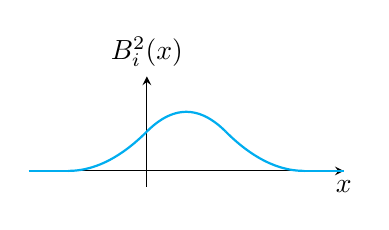
\begin{tikzpicture}
     % draw the axis
     \draw[eaxis] (-1.5,0) -- (2.5,0) node[below] {$x$};
     \draw[eaxis] (0,-0.2) -- (0,1.2) node[above] {$B_i^2(x)$};
     % draw the function (piecewise)
     \draw[elegant,domain=-1.5:-1] plot(\x,0);
     \draw[elegant,domain=-1:0] plot(\x,{(\x+1)^2/2});
     \draw[elegant,domain=0:1] plot(\x,{(\x+1)*(1-\x)/2+(2-\x)*\x/2});
     \draw[elegant,domain=1:2] plot(\x,{(2-\x)^2/2});
     \draw[elegant,domain=2:2.5] plot(\x,0);
    \end{tikzpicture}
  \end{center}
  \end{enumerate}
\end{solution}

\vspace{1.5em}

\begin{problem}
  Verify Theorem 3.32 algebraically for the case of $n=2$, i.e.
  \begin{equation*}
    (t_{i+2}-t_{i-1})[t_{i-1},t_i,t_{i+1},t_{i+2}](t-x)_+^2=B_i^2(x).
  \end{equation*}
\end{problem}

\begin{solution}
  For $x\in(t_{i-1},t_i]$, by Lagrange's formula we have:
  \begin{align*}
    [t_{i-1},t_i,t_{i+1},t_{i+2}](t-x)_+^2=&\frac{(t_i-x)^2}{(t_i-t_{i-1})(t_{i}-t_{i+1})(t_i-t_{i+2})}+\frac{(t_{i+1}-x)^2}{(t_{i+1}-t_{i-1})(t_{i+1}-t_{i})(t_{i+1}-t_{i+2})}\\
    &+\frac{(t_{i+2}-x)^2}{(t_{i+2}-t_{i-1})(t_{i+2}-t_{i})(t_{i+2}-t_{i+1})}\\
    =&\frac{(x-t_{i-1})^2}{(t_{i+2}-t_{i-1})(t_{i+1}-t_{i-1})(t_i-t_{i-1})}=\frac{B_i^2(x)}{t_{i+2}-t_{i-1}}
  \end{align*}
  For $x\in(t_{i},t_{i+1}]$, by Lagrange's formula we have:
  \begin{align*}
    [t_{i-1},t_i,t_{i+1},t_{i+2}](t-x)_+^2=&\frac{(t_{i+1}-x)^2}{(t_{i+1}-t_{i-1})(t_{i+1}-t_{i})(t_{i+1}-t_{i+2})}+\frac{(t_{i+2}-x)^2}{(t_{i+2}-t_{i-1})(t_{i+2}-t_{i})(t_{i+2}-t_{i+1})}\\
    =&\frac{B_i^2(x)}{t_{i+2}-t_{i-1}}
  \end{align*}
  For $x\in(t_{i+1},t_{i+2}]$, by Lagrange's formula we have:
  \begin{align*}
    [t_{i-1},t_i,t_{i+1},t_{i+2}](t-x)_+^2=&\frac{(t_{i+2}-x)^2}{(t_{i+2}-t_{i-1})(t_{i+2}-t_{i})(t_{i+2}-t_{i+1})}\\
    =&\frac{B_i^2(x)}{t_{i+2}-t_{i-1}}
  \end{align*}
  Hence we verified
  \begin{equation*}
    (t_{i+2}-t_{i-1})[t_{i-1},t_i,t_{i+1},t_{i+2}](t-x)_+^2=B_i^2(x)
  \end{equation*}
  in the support of $B_i^2(x)$. And clearly, the equation is also right when $B_i^2(x)$ vanishes.
\end{solution}

\vspace{1.5em}

\begin{problem}
  Scaled integral of B-splines.

  Deduce from the Theorem on deriviates of B-splines that the scaled integral of a B-spline $B_i^n(x)$ over its support is independent of its index $i$ even if the spacing of the knots is not uniform.
\end{problem}

\begin{solution}
  By the Theorem on derivates of B-splines, we have
  \begin{equation*}
    \frac{\text{d}}{\text{d}x}B_i^{n+1}(x)=\frac{(n+1)B_i^{n}(x)}{t_{i+n}-t_{i-1}}-\frac{(n+1)B_{i+1}^{n}(x)}{t_{i+n+1}-t_i} ,\qquad n=1,2,...
  \end{equation*}
  Integral to both side, we have:
  \begin{equation*}
    \int_{t_{i-1}}^{t_{i+n+1}}\frac{\text{d}}{\text{d}x}B_i^{n+1}(x) \text{d}x=\int_{t_{i-1}}^{t_{i+n+1}}\frac{(n+1)B_i^{n}(x)}{t_{i+n}-t_{i-1}}-\frac{(n+1)B_{i+1}^{n}(x)}{t_{i+n+1}-t_i}\text{d} x,\qquad n=1,2,...
  \end{equation*}
  For the left side, we have:
  \begin{equation*}
    \text{LHS}=B_i^{n+1}(t_{i+n+1})-B_i^{n+1}(t_{i-1})=0-0=0.
  \end{equation*}
  For the right side, we have:
  \begin{equation*}
    \text{RHS}=(n+1)\left(\int_{t_{i-1}}^{t_{i+n}}\frac{B_i^{n}(x)}{t_{i+n}-t_{i-1}} \text{d}x-\int_{t_{i}}^{t_{i+n+1}}\frac{B_{i+1}^{n}(x)}{t_{i+n+1}-t_{i}} \text{d}x\right)
  \end{equation*}
  Then we got
  \begin{equation*}
    \int_{t_{i-1}}^{t_{i+n}}\frac{B_i^{n}(x)}{t_{i+n}-t_{i-1}} \text{d}x=\int_{t_{i}}^{t_{i+n+1}}\frac{B_{i+1}^{n}(x)}{t_{i+n+1}-t_{i}} \text{d}x
  \end{equation*}
  Hence the scaled integral of $B_i^n(x)$ over its support is independent of $i$.
\end{solution}

\vspace{1.5em}

\begin{problem}
  Symmetric Polynomials.

  We have a theorem on expressing complete symmetric polynomials as divided difference of monomials.
  \begin{enumerate}[(a)]
    \item Verify this theorem for $m=4$ and $n=2$ by working out the table of divided difference and comparing the result to the definition of complete symmetric polynomials.
    \item Prove this theorem by the lemma on the recursive relation on complete symmetric polynomials.
  \end{enumerate}
\end{problem}

\begin{solution}
  \begin{enumerate}[(a)]
    \item By the definition,
    \begin{equation*}
      \tau_2(x_i,x_{i+1},x_{i+2})=x_i^2+x_{i+1}^2+x_{i+2}^2+x_ix_{i+1}+x_ix_{i+2}+x_{i+1}x_{i+2}.
    \end{equation*}
    Make a table of divided difference as following.
    \begin{table}[H]
      \centering
      \begin{tabular}{l|lll}
      $x_i$     & $x_i^4$     &                                          &                                                                                                 \\
      $x_{i+1}$ & $x_{i+1}^4$ & $(x_{i+1}^2+x_{i}^2)(x_{i+1}+x_{i})$     &                                                                                                 \\
      $x_{i+2}$ & $x_{i+2}^4$ & $(x_{i+2}^2+x_{i+1}^2)(x_{i+2}+x_{i+1})$ & $\frac{(x_{i+2}^2+x_{i+1}^2)(x_{i+2}+x_{i+1})-(x_{i+1}^2+x_{i}^2)(x_{i+1}+x_{i})}{x_{i+2}-x_i}$
      \end{tabular}
    \end{table}
    Then the result follows from 
    \begin{align*}
      &\frac{(x_{i+2}^2+x_{i+1}^2)(x_{i+2}+x_{i+1})-(x_{i+1}^2+x_{i}^2)(x_{i+1}+x_{i})}{x_{i+2}-x_i}\\
      =&\frac{(x_{i+2}^3-x_i^3)+x_{i+1}(x_{i+2}^2-x_i^2)+x_{i+1}^2(x_{i+2}-x_i)}{x_{i+2}-x_i}\\
      =&(x_{i+2}^2+x_{i+2}x_i+x_i^2)+x_{i+1}(x_{i+2}+x_i)+x_{i+1}^2\\
      =&\tau_2(x_i,x_{i+1}+x_{i+2}).
    \end{align*}

    \item By the lemma on recursive relations of complete symmetric polynomials, we have
    \begin{align*}
      &(x_{i+n+1}-x_i)\tau_{m-n-1}(x_i,...,x_{i+n+1})\\
      =&\tau_{m-n}(x_i,...,x_{i+n+1})-\tau_{m-n}(x_i,...,x_{i+n})-x_i\tau_{m-n-1}(x_i,...,x_{i+n+1})\\
      =&\tau_{m-n}(x_{i+1},...,x_{i+n+1})+x_i\tau_{m-n-1}(x_i,...,x_{i+n+1})-\tau_{m-n}(x_i,...,x_{i+n})-x_i\tau_{m-n-1}(x_i,...,x_{i+n+1})\\
      =&\tau_{m-n}(x_{i+1},...,x_{i+n+1})-\tau_{m-n}(x_i,...,x_{i+n}).
    \end{align*}
    Now we prove the theorem by induction. For $n=0$, clearly
    \begin{equation*}
      \tau_m(x_i)=[x_i]x^m=x_i^m.
    \end{equation*}
    Now we suppose the theorem is true for some $0\leq n<m$. Then for $n+1$, we have
    \begin{align*}
      \tau_{m-n-1}(x_i,...,x_{i+n+1})&=\frac{\tau_{m-n}(x_{i+1},...,x_{i+n+1})-\tau_{m-n}(x_i,...,x_{i+n})}{x_{i+n+1}-x_{i}}\\
      &=\frac{[x_{i+1},...,x_{i+n+1}]x^m-[x_i,...,x_{i+n}]}{x_{i+n+1}-x_{i}}\\
      &=[x_i,...,x_{i+n+1}]x^m
    \end{align*}
    Then the theorem is proved by induction.
  \end{enumerate}
\end{solution}

\chapter{Computer Arithmetic}

\begin{problem}
  Convert the decimal integer $477$ to a normalized FPN with $\beta=2$.
\end{problem}

\begin{solution}
  $477=(111011101)_2=(1.11011101)_2\times 2^8.$
\end{solution}

\vspace{1em}

\begin{problem}
  Convert the decimal fraction $\frac{3}{5}$ to a normalized FPN with $\beta=2$.
\end{problem}

\begin{solution}
  Calculate by the following table.
  \begin{table}[H]
    \centering
    \begin{tabular}{ccc}
    Arithmetic                        & Decimal Part  & Integer Part \\ \hline
    $\frac{3}{5}\times 2=\frac{6}{5}$ & $\frac{1}{5}$ & $1$          \\
    $\frac{1}{5}\times 2=\frac{2}{5}$ & $\frac{2}{5}$ & $0$          \\
    $\frac{2}{5}\times 2=\frac{4}{5}$ & $\frac{4}{5}$ & $0$          \\
    $\frac{4}{5}\times 2=\frac{8}{5}$ & $\frac{3}{5}$ & $1$          \\
    $\vdots$                          & $\vdots$      & $\vdots$    
    \end{tabular}
  \end{table}

  Hence we got that
  \begin{equation*}
    \frac{3}{5}=(1.0011001\cdots)_2\times 2^{-1}
  \end{equation*}
\end{solution}

\vspace{1em}

\begin{problem}
  Let $x=\beta^e,\;e\in\mathbb{Z},\;L<e<U$ be a normalized FPN in $\mathbb{F}$ and $x_L,x_R\in \mathbb{F}$ the two normalized FPNs adjacent to $x$ such that $x_L<x<x_R$. Prove $x_R-x=\beta(x-x_L)$.
\end{problem}

\begin{solution}
  We represent $x,x_L,x_R$ in the form of normalized FPN as following.
  \begin{align*}
    x&=(1.00\cdots 0)_\beta \times \beta^{e}\\
    x_L&=([\beta-1].[\beta-1]\cdots [\beta-1])_\beta \times \beta^{e-1}\\
    x_R&=(1.00\cdots 01)_\beta \times \beta^{e}
  \end{align*}

  And hence we have:
  \begin{align*}
    x_R-x&=(0.00\cdots 01)_\beta\times \beta^{e}=\beta^{e-p+1}\\
    x-x_L&=(0.00\cdots 01)_\beta\times \beta^{e-1}=\beta^{e-p}
  \end{align*}

  That is $x_R-x=\beta(x-x_L)$.
\end{solution}

\vspace{1em}

\begin{problem}
  By reusing your result of II, find out the two normalized FPNs adjacent to $x=\frac{3}{5}$ under the IEEE 754 single-precision protocol. What is $\text{fl}(x)$ and the relative roundoff error?
\end{problem}

\begin{solution}
  Recall that $x=(1.0011001\cdots)_2\times 2^{-1}$, find $x_L$ and $x_R$ under IEEE 754 single-precision protocol:
  \begin{align*}
    x_L &= (1.0011001\;10011001\;1001100)_2\times 2^{-1},\\
    x_R &= (1.0011001\;10011001\;1001101)_2\times 2^{-1}.
  \end{align*}

  We calculate that:
  \begin{align*}
    x-x_L &= (1.10011001\cdots)_2\times 2^{-23}=\frac{8}{5} \times 2^{-23},\\
    x_R-x_L &= 2^{-22},\\
    x_R-x&=(x_R-x_L)-(x-x_L)=2^{-22}-\frac{8}{5} \times 2^{-23}=\frac{2}{5}\times 2^{-23}.
  \end{align*}

  Clearly that $x_R-x<x-x_L$, hence $\text{fl}(x)=x_R$ and the relative roundoff error is $\frac{|x_R-x|}{|x|}=\frac{2}{3}\times 2^{-23}$.
\end{solution}

\begin{problem}
  If the IEEE 754 single-precision protocol did not round off numbers to the nearest, but simply dropped excess bits, what would the unit roundoff be?
\end{problem}

\begin{solution}
  It would be $\epsilon_u^*=\epsilon_M=\beta^{1-p}=2^{-23}$.
  
  To prove it, we should prove that for $x\in\mathcal{R(F)}$, we have
  \begin{equation}
    \text{fl}^*(x)=x(1+\delta), \qquad |\delta|<\epsilon_u^*
  \end{equation}

  where $\text{fl}^*(x)$ is the approximate of $x$ got by the discription of the problem.

  we could find $x_L,x_R\in\mathcal{F}$ s.t.

  \begin{itemize}
    \item $x_L$ and $x_R$ are adjacent.
    \item $x_L\leq x\leq x_R$.
  \end{itemize}

  If $x=x_L$ or $x=x_R$, then $\text{fl}^*(x)-x=0$ and (4.1) clearly holdes. Otherwise $x_L<x<x_R$. Then Lemma 4.23, Definition 4.22 yield
  \begin{equation*}
    |\text{fl}^*(x)-x|\leq |x_R-x_L|\leq \epsilon_u^*\min(|x_L|,|x_R|)< \epsilon_u^*|x|.
  \end{equation*}

  which yields (4.1). And the upper bound of the error can be reached as $x\to x_{R-}$. Hence $\epsilon_u^*$ is the unit roundoff.
\end{solution}

\vspace{1em}

\begin{problem}
  How many bits of precision are lost in the subtraction $1-\cos x$ when $x=\frac{1}{4}$?
\end{problem}

\begin{solution}
  For $x=\frac{1}{4}$, we know that $1>\cos x$, hence by the theorem on the loss of most significant digits, we should calculate:
  \begin{equation*}
    1-\frac{\cos x}{1}=0.0310875783\cdots \in [2^{-6},2^{-5}].
  \end{equation*}
  
  (The result above is calculated with \verb|long double|, which is accurate enough.)

  Hence we lost at most $6$ and at least $5$ significant bits.
\end{solution}

\vspace{1em}

\begin{problem}
  Suggest at least two ways to compute $1-\cos x$ to avoid catastrophic cancellation caused by subtraction.
\end{problem}

\begin{solution}
  \begin{enumerate}[(1)]
    \item We can use Taylor series:
    \begin{align*}
      1-\cos x&=1-\left(1-\frac{x^2}{2!}+\frac{x^4}{4!}-\frac{x^6}{6!}+\cdots\right)\\
      &=\frac{x^2}{2!}-\frac{x^4}{4!}+\frac{x^6}{6!}-\cdots.
    \end{align*}

    \item We can use sum-to-product identities:
    \begin{align*}
      1-\cos x= \cos 0- \cos x= 2\sin^2\left(\frac{x}{2}\right).
    \end{align*}
  \end{enumerate}
\end{solution}

\vspace{1em}

\begin{problem}
  What are the condition numbers of the following functions? Where are they large?
  \begin{itemize}
    \item $f_1(x)=(x-1)^\alpha$,
    \item $f_2(x)=\ln x$,
    \item $f_3(x)=e^x$,
    \item $f_4(x)=\arccos x$.
  \end{itemize}
\end{problem}

\begin{solution}
  \begin{itemize}
    \item We should discuss the value of $\alpha$.
    \begin{enumerate}[(i)]
      \item $\alpha\neq 0$. The condition number of $f_1$ is $C_{f_1}(x)=\left|\frac{xf'_1(x)}{f_1(x)}\right|=\left|\frac{\alpha x(x-1)^{\alpha-1}}{(x-1)^\alpha}\right|=\left|\frac{\alpha x}{x-1}\right|.$

      Hence $C_{f_1}(x)\to +\infty$ as $x\to 1$.
      \item $\alpha=0$. The condition number of $f_1$ is $C_{f_1}(x)=\left|\frac{xf'_1(x)}{f_1(x)}\right|=\left|\frac{0}{1}\right|=0.$

      Hence $C_{f_1}(x)$ will never be large.
    \end{enumerate}
    \item The condition number of $f_2$ is $C_{f_2}(x)=\left|\frac{xf'_2(x)}{f_2(x)}\right|=\left|\frac{x \cdot \frac{1}{x}}{\ln x}\right|=\left| \frac{1}{\ln x} \right|.$
    
    Hence $C_{f_2}(x)\to +\infty$ as $x\to 0_+$.
    \item The condition number of $f_3$ is $C_{f_3}(x)=\left|\frac{xf'_3(x)}{f_3(x)}\right|=\left|\frac{x e^x}{e^x}\right|=\left|x \right|.$

    Hence $C_{f_3}(x)\to +\infty$ as $x\to \pm \infty$.
    \item The condition number of $f_4$ is $C_{f_4}(x)=\left|\frac{xf'_4(x)}{f_4(x)}\right|=\left| \frac{x}{\sqrt{1-x^2}\arccos x} \right|$

    Hence $C_{f_4}(x)\to +\infty$ as $x\to \pm 1$.
  \end{itemize}
\end{solution}

\vspace{1em}

\begin{problem}
  Consider the function $f(x)=1-e^{-x}$ for $x\in[0,1]$.
  \begin{itemize}
    \item Show that $C_f(x)\leq 1$ for $x\in[0,1]$.
    \item Let $A$ be the algorithm that evaluates $f(x)$ for the machine number $x\in\mathbb{F}$. Assume that the exponential function is computed with relative error within machine roundoff. Estimate $\text{cond}_A(x)$ for $x\in[0,1]$.
    \item Plot $\text{cond}_f(x)$ and the estimated upper bound of $\text{cond}_A(x)$ as a function of $x$ on $[0,1]$. Discuss your results.
  \end{itemize}
\end{problem}

\begin{solution}
  \begin{enumerate}[(1)]
    \item The condition number of $f$ is $C_f(x)=\left|\frac{xe^{-x}}{1-e^{-x}}\right|=\left|\frac{x}{e^x-1}\right|.$

    Notice that $C_f(x)$ decreases in $x\in[0,1]$, and $\lim\limits_{x\to 0} C_f(x)=1$. Hence $C_f(x)\leq 1$ for $x\in[0,1]$.
    \item See that
    \begin{equation*}
      \epsilon_u > |f_A(x)-f(x)|=|f(x_A)-f(x)|=|f'(\xi)|\cdot|x-x_A|,\quad \text{for} \;\xi \; \text{between} \; x \; \text{and} \; x_A.
    \end{equation*}
    So we have
    \begin{equation*}
      |x-x_A|< \frac{\epsilon_u}{|f'(\xi)|}=\frac{\epsilon_u}{e^{-\xi}}\leq e\epsilon_u.
    \end{equation*}
    Hence by the definition, 
    \begin{equation*}
      \text{cond}_A(x)=\frac{1}{\epsilon_u}\min_{\{x_A\}}\frac{|x-x_A|}{x}< \frac{e}{x}.
    \end{equation*}
    \item See the figure of $C_f(x)$ and the upper bound of $\text{cond}_A(x)$ here.
    \tikzset{global scale/.style={
      scale=#1,
      every node/.append style={scale=#1}
      }
    }
    \begin{center}
      \begin{tikzpicture}[global scale = 0.8]
        \begin{axis}[
            axis lines=middle,
            samples=51,
      %       grid,                
      %      thick,
            domain=0.2:1,
            legend pos=outer north east,
            smooth,
        ]
        \addplot+[no marks]{\x/(e^\x-1)};
        \addplot+[no marks]{e/\x};
        \addlegendentry{$\text{cond}_f(x)$}
        \addlegendentry{upper bound of $\text{cond}_A(x)$}
        \end{axis}
      \end{tikzpicture}
    \end{center}

    The upper bound of $\text{cond}_A(x)$ goes large as $x\to 0_+$, which means calculating $f$ with algorithm $A$ as $x$ is small will cause catastrophic cancellation.
  \end{enumerate}
\end{solution}

\vspace{1em}

\begin{problem}
  The math problem of root finding for a polynomial
  \begin{equation}
    q(x)=\sum_{i=0}^n a_ix^i, \quad a_n=1,a_0\neq 0,a_i\in \mathbb{R}
  \end{equation}
  can be considered as a vector function $f:\mathbb{R}^n \to \mathbb{C}$:
  \begin{equation*}
    r=f(a_0,a_1,...,a_{n-1}).
  \end{equation*}

  Derive the componentwise condition number of $f$ base on the 1-norm. For the Wilkinson example, conpute your condition number, and compare your result with that in the Wilkinson Example. What does the comparision tell you?
\end{problem}

\begin{solution}
  Notice that $r$ satisfies equation
  \begin{equation*}
    \sum_{i=0}^n a_ir^i = 0.
  \end{equation*}
  
  Compute partial differetial to each side, we have
  \begin{equation*}
    r^j + \sum_{i=0}^n ia_ir^{i-1}\frac{\partial r}{\partial a_j} = 0, \qquad j=1,2,...,n-1.
  \end{equation*}

  That implies 
  \begin{equation*}
    \nabla r = -\frac{(1, r, ..., r^{n-1})}{q'(r)}.
  \end{equation*}

  Hence we have
  \begin{equation*}
    \text{cond}_f(\mathbf{a})=\frac{||\mathbf{a}||_1\;||\nabla r||_1}{|r|}=\frac{\sum_{i=1}^{n-1} |a_i|\cdot\sum_{i=0}^{n-1} |r|^i}{\left|\sum_{i=0}^n ia_ir^i\right|} \left(\geq \frac{\sum_{i=1}^{n-1} |a_ir^i|}{\left|\sum_{i=0}^n ia_ir^i\right|}\right)
  \end{equation*}

  In Wilkinson example, $q(x)=\prod_{i=1}^n (x-i)$, $r=n$ is a root. Then we have
  \begin{equation*}
    \sum_{i=0}^{n-1}|a_nr^i| \geq -\sum_{i=0}^{n-1} a_ir^i = r^n = n^n,
  \end{equation*}
  and
  \begin{equation*}
    \left|\sum_{i=0}^n ia_ir^i\right| = |r| \cdot |q'(r)| = n|q'(n)| < n^2 n!.
  \end{equation*}

  Hence we have $\text{cond}_f(\mathbf{a})\geq \frac{n^{n-2}}{n!}$, which goes $+\infty$ as $n\to \infty$. It supports the Wilkinson Example. And it tells us that finding the root of high-order polynomial equation is very hard.
\end{solution}

\vspace{1em}

\begin{problem}
  Suppose the division of two FPNs is calculated in a register of precision $2p$. Give an example that contradicts the conclusion of the model of machine arithmetic.
\end{problem}

\begin{solution}
  Consider the FPN system: $\beta=2, p=2, L=-1, U=1$. The number:
  \begin{equation*}
    a=(1.0)_2\times 2^{0},\quad b=(1.1)_2\times 2^{0}.
  \end{equation*}

  We have the theoretical result:
  \begin{equation*}
    \frac{a}{b}=\frac{2}{3}=(0.101010\cdots)_2.
  \end{equation*}

  If calculating in a register with precision $2p=4$, then:
  \begin{equation*}
    \text{fl}\left(\frac{a}{b}\right)=\text{fl}((0.101)_2)=(0.10)_2\times 2^{0}=0.5
  \end{equation*}

  The relative error is
  \begin{equation*}
    \left|\frac{0.5}{\frac{2}{3}}-1\right|=0.25
  \end{equation*}

  And the machine precision is
  \begin{equation*}
    \epsilon_u=2^{-2}=0.25
  \end{equation*}

  So the result contradicts to the model of machine arithmetic.

\end{solution}

\begin{problem}
  If the bisection method is used in single precision FPNs of IEEE 754 starting with the interval $[128,129]$, can we compute the root with absolute accuracy $<10^{-6}$? Why?
\end{problem}

\begin{solution}
  In this system, $\epsilon_M=2^{-23}$. Hence the distance of two adjacent floating numbers in $[128,129]$ is
  \begin{equation*}
    2^7\epsilon_M=2^{-16}\approx 1.5259\times 10^{-5}>2\times 10^{-6}.
  \end{equation*}

  Hence we can't compute the root with absolute accuracy less than $10^{-6}$.
\end{solution}

\vspace{1em}

\begin{problem}
  In fitting a curve by cubic splines, one gets inaccurate results when the distance between two adjacent points is much smaller than those of other adjacent pairs. Use the condition number of a matrix to explain this phenomenon.
\end{problem}

\begin{solution}
  Consider calculate $s(x)=ax^3+bx^2+cx+d$ on $[x_i,x_{i+1}]$ by $s(x_i),s(x_{i+1}),s'(x_i),s'(x_{i+1})$. We should solve a linear equation where the coefficient matrix is
  \begin{equation*}
    \begin{pmatrix}
      x_i^3 & x_i^2 & x_i & 1\\
      x_{i+1}^3 & x_{i+1} ^2 & x_{i+1} & 1\\
      3x_i^2 & 2x_i & 1 & 0\\
      3x_{i+1}^2 & 2x_{i+1} & 1 & 0
    \end{pmatrix}.
  \end{equation*}

  It has large condition number when $x_i$ and $x_{i+1}$ are close enough. So the result will be very inaccurate.
\end{solution}

\end{document}